\section {Method and material}

We employed a hierarchical learning approach to classify the taxonomy of a virus based on its DNA sequence. Our method begins with an initial classifier that predicts the order of the virus. Once the order is identified, a second classifier is used to determine the family. Although further classifiers could be applied to predict the genus and species of the virus, this research focuses primarily on evaluating the effectiveness of the classifier. Therefore, we limited our study to the two viral orders, Martellivirales and Tymovirales.

After the order is predicted, the corresponding family classifier is applied to identify the specific family of the virus within that order. To maintain robust classification performance, we excluded families with fewer than five species and species with sequence lengths shorter than 100 base pairs.

This hierarchical approach enables accurate virus classification from DNA sequences, offering valuable insights into the virus’s characteristics and potential impact. By dividing the classification process into smaller, targeted steps, we effectively manage the complexity of viral taxonomy, enhancing our capacity to study and address viral threats.

In the following subsections, we discuss the dataset used, data preprocessing, and the machine learning model applied in this study.

\subsection{Dataset}
\label{sec:obj:det}

The dataset for this research was sourced from the National Center for Biotechnology Information (NCBI) RefSeq database, which offers high-quality, curated sequences that have been reviewed and annotated by experts, ensuring accuracy and reliability. RefSeq provides a single, well-characterized reference sequence for each virus, minimizing redundancy and simplifying data interpretation. Additionally, each RefSeq entry has a stable identifier, facilitating consistent referencing and reporting.

To acquire the relevant sequences, we used the latest Virus Metadata Resource (VMR) spreadsheet available from the International Committee on Taxonomy of Viruses (ICTV) at https://ictv.global/vmr/current, as well as on the associated GitHub repository. This file contains comprehensive metadata for all viruses. Using RefSeq accession numbers listed in the VMR spreadsheet, we downloaded the DNA sequences for the taxa of interest in this study.

In our research, we focused on the classification of viruses within the Alsuviricetes class, belonging to the Kitrinoviricota phylum, which is part of the Orthornavirae kingdom in the Orthornavirae realm. We developed a hierarchical classification approach, starting by categorizing viruses into two orders: Martellivirales and Tymovirales.

Subsequently, we employed specialized classifiers to distinguish among the families within each order. For the Martellivirales order, we differentiated between the families Virgaviridae, Closteroviridae, Bromoviridae, Togaviridae, Endornaviridae, and Solspiviridae. For the Tymovirales order, we further classified viruses into Betaflexiviridae, Alphaflexiviridae, and Tymoviridae families. This multi-level classification approach allowed us to systematically analyze and categorize the viral sequences with a high degree of precision. Table \ref{table:species_counts} provides an overview of the number of families and species in each order. This structured dataset enabled us to perform a comprehensive and precise classification of viral sequences across the chosen taxonomic levels.

\begin{table}[tb]
\centering
\begin{tabular}{| l | l | l |}
\hline
\textbf{Order} & \textbf{Family} & \textbf{Species} \\
\hline
\multirow{5}{*}{Martellivirales} & Virgaviridae & 56 \\
                                  & Closteroviridae & 54 \\
                                  & Bromoviridae & 38 \\
                                  & Togaviridae & 37 \\
                                  & Endornaviridae & 31 \\
\hline
\multirow{3}{*}{Tymovirales}     & Betaflexiviridae & 125 \\
                                  & Alphaflexiviridae & 65 \\
                                  & Tymoviridae & 34 \\
\hline
\end{tabular}
\caption{Number of families and species in each order.}
\label{table:species_counts}
\end{table}

\subsection{Hierarchical Classification}

\begin{figure}[t]
\begin{centering}
		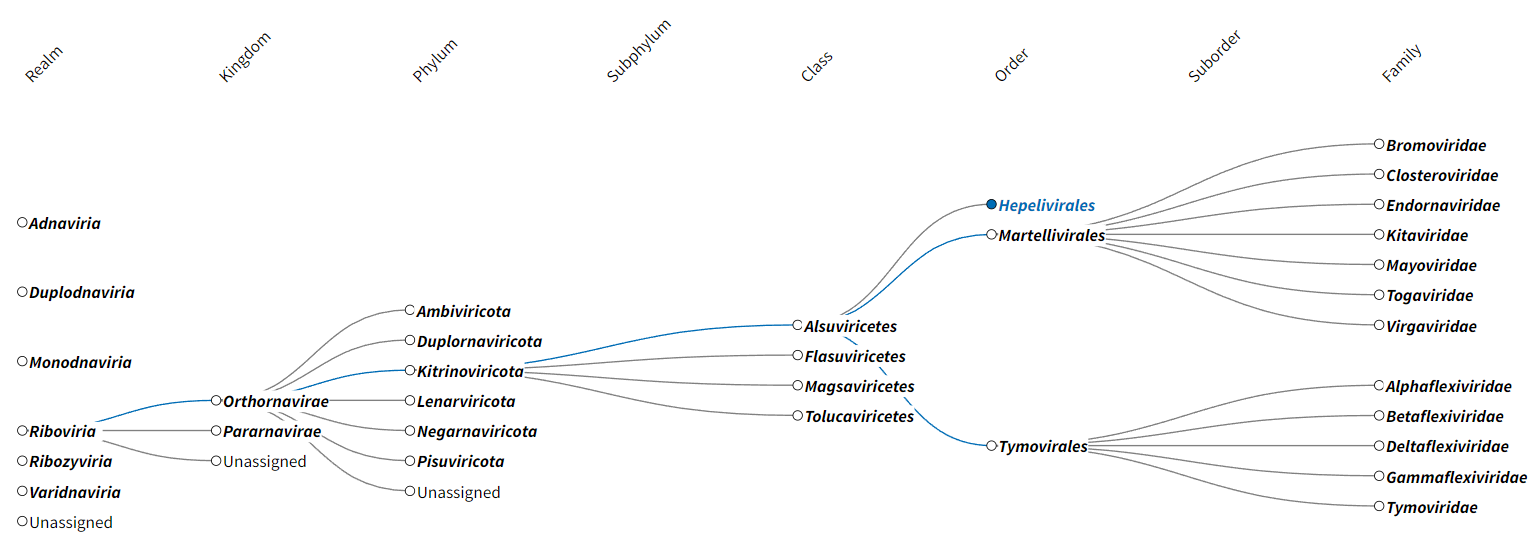
\includegraphics[width=.48\textwidth]{Figures/heirarchy_IVT.png}
	\caption{distribution  }
\label{fig:distr}
\end{centering}
\end{figure}

The ICTV scheme organizes classes into a hierarchical taxonomic tree. From the highest to the deepest levels, these are: Realm, Kingdom, Phylum, Subphylum, Class, Order, Family, Subfamily, Genus, and Species. In hierarchical classification, our aim is to predict a set of hierarchically structured classes for each virus. A comprehensive review of hierarchical classification is available in [81][82]. Hierarchical classifiers can be categorized into three types based on how they utilize hierarchical information: the flat classifier approach, the local classifier approach, and the global classifier (big-bang) strategy. In this paper, we adopted the Local Classifiers per Parent Node (LCPN) approach. This approach reduces the number of classifiers compared to the Local Classifiers per Node (LCN) method, while still capturing hierarchical information. Unlike the flat classifier approach, LCPN explicitly incorporates the class hierarchy. Moreover, it is more intuitive and simpler than the big-bang classification strategy.










